\documentclass[10pt, aspectratio=169]{beamer} %
\usetheme{Singapore}

\usepackage{bookmark}
\usepackage{graphicx}
\usepackage[english]{babel}
\usepackage[utf8]{inputenc}
\usepackage[T1]{fontenc}
\usepackage{amsmath}
\usepackage{color}
\usepackage{listings}
\usepackage{tabularx}
\usepackage{amssymb}
\usepackage{lmodern}

\usepackage{hyperref}
\hypersetup{colorlinks=true, urlcolor=blue}

\DeclareMathOperator*{\minimize}{minimize} %in preamble
 
\newcommand{\N}{{\mathbb{N}}}
\newcommand{\I}{{\bf I}}
\newcommand{\C}{{\bf C}}
\newcommand{\A}{{\bf A}}
\newcommand{\T}{{\bf T}}
\newcommand{\g}{{\bf g}}
\newcommand{\e}{{\bf e}}
\newcommand{\ab}{{\bf a}}
\newcommand{\ba}{{\bf b}}
\newcommand{\Z}{{\mathbb{Z}}}
\newcommand{\R}{{\mathbb{R}}}
\newcommand{\mbf}{\mathbf}
\newcommand{\bs}{\boldsymbol}
\newcommand{\cc}{{\bf c}}
\newcommand{\su}{{\sum_{n=0}^{N-1}}}

\newcommand{\argmax}{\mathop{\text{arg\;max}}}
\newcommand{\argmin}{\mathop{\text{arg\;min}}}

\newcommand{\HH}{{\bf H}}
\newcommand{\thb}{\boldsymbol{\theta}}
\newcommand{\w}{{\bf w}}
\newcommand{\Sigb}{\boldsymbol{\Sigma}}
\newcommand{\mub}{\boldsymbol{\mu}}
\newcommand{\alb}{\boldsymbol{\alpha}}

\newcommand{\s}{{\bf s}}
\newcommand{\SB}{{\bf S}}

\definecolor{blue}{RGB}{32,32,255}
\graphicspath{{./images/}}

\newcommand{\h}{{\bf h}}
\newcommand{\rr}{{\bf r}}
\newcommand{\X}{{\bf X}}
\newcommand{\x}{{\bf x}}
\newcommand{\y}{{\bf y}}
\newcommand{\p}{{\bf p}}
\newcommand{\E}{{\bf E}}
\newcommand{\U}{{\bf U}}
\newcommand{\V}{{\bf V}}
\newcommand{\f}{{\bf f}}
\newcommand{\var}{{\mathop{\text{var}}}}

\newcommand{\F}{{\cal F}}
\newcommand{\leveys}{0.75\textwidth}
\newcommand{\etaisyys}{0.25\textwidth}

\newcommand{\sinc}{\mathop{\text{sinc}}}
\newcommand{\esim}{\em}

\newcommand{\modulo}{\operatorname{mod}}

\setbeamertemplate{frametitle continuation}[from second] 

\renewcommand{\insertcontinuationtext}{}

\setbeamertemplate{frametitle}
{
	\vspace*{0.7cm} \vbox{\insertframetitle}
}

\usecolortheme{default}

\setbeamertemplate{mini frames}{}
\renewcommand*{\slideentry}[6]{}
\setbeamertemplate{frametitle}{
    \vspace*{0.2cm}
    \insertframetitle
}

\title{Pattern Recognition and Machine Learning}
\subtitle{Slide Set 5: Ensemble Methods}
\author{Heikki Huttunen\\
heikki.huttunen@tut.fi}
\institute{Department of Signal Processing\\Tampere University of Technology}
\date{January 2017}

\begin{document}

\maketitle

\lstdefinestyle{mystyle}{
  belowcaptionskip=1\baselineskip,
  breaklines=true,
  frame=single,
  xleftmargin=\parindent,
  language=Python,
  showstringspaces=false,
  basicstyle=\tiny\ttfamily,
  keywordstyle=\bfseries\color{green!40!black},
  commentstyle=\itshape\color{purple!40!black},
  identifierstyle=\color{blue},
  stringstyle=\color{orange},
  moredelim=**[is][\color{red}]{@}{@},
}

\lstset{language=Python,style=mystyle} 

\begin{frame}
\vspace*{2cm}
\centerline{\Large RANDOM FOREST}
\centerline{(and other ensemble methods)}
\end{frame}

\begin{frame}{Random Forest}
\begin{columns}
\column{0.7\textwidth}
\begin{itemize}
\item Random forest (RF) is popular tree based classifier, proposed by Breiman in 1993.
\item The RF is based on a collection of \emph{decision trees}.
\item A decision tree is a straightforward if-then-else-like diagram
that combines individual attributes into a decision.
\item Decision trees are easily trained to learn the data.
\item For example, the tree on the right predicts the time of year from the following
measured attributes:
$\{\text{Temperature}, \text{Snow}, \text{Rain}, \text{Sunny}\}$.
\end{itemize}
\column{0.3\textwidth}
\centerline{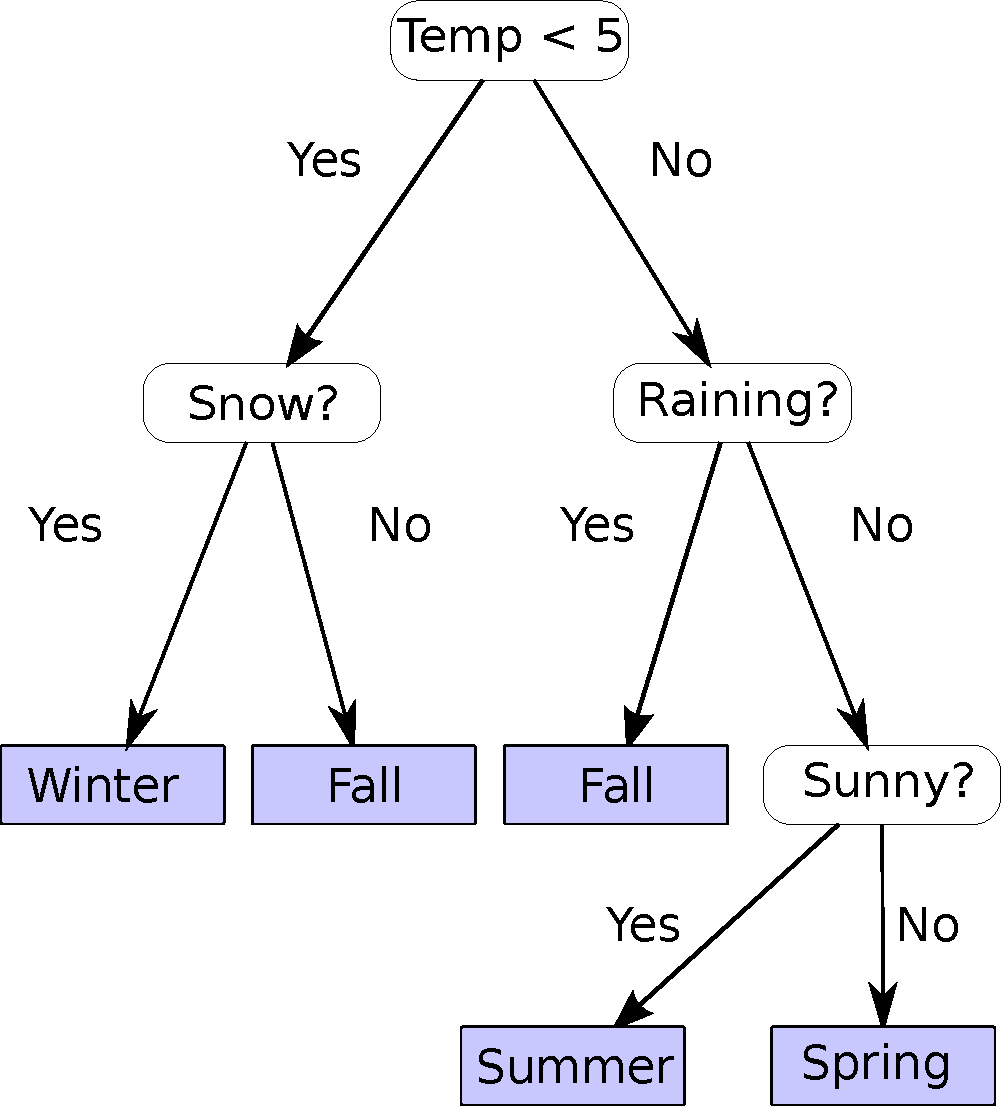
\includegraphics[width=1.2\columnwidth]{DecisionTree.pdf}}
\end{columns}
\end{frame}

\begin{frame}{Random Forest}
\begin{columns}
\column{0.7\textwidth}
\begin{itemize}
\item The problem of decision trees is that they \emph{overlearn} the data,
\emph{i.e.,} the training data is memorized with a poor ability to generalize.
\item With no restrictions, the DT will have one root-leaf-path per sample, which
is essentially same as nearest neighbor.
\item RF avoids this by training many "imperfect" trees.
\item Each tree is trained with a subset of samples and a subset of
features, \emph{i.e.,} some of the attributes are hidden from the training.
\end{itemize}
\column{0.3\textwidth}
\centerline{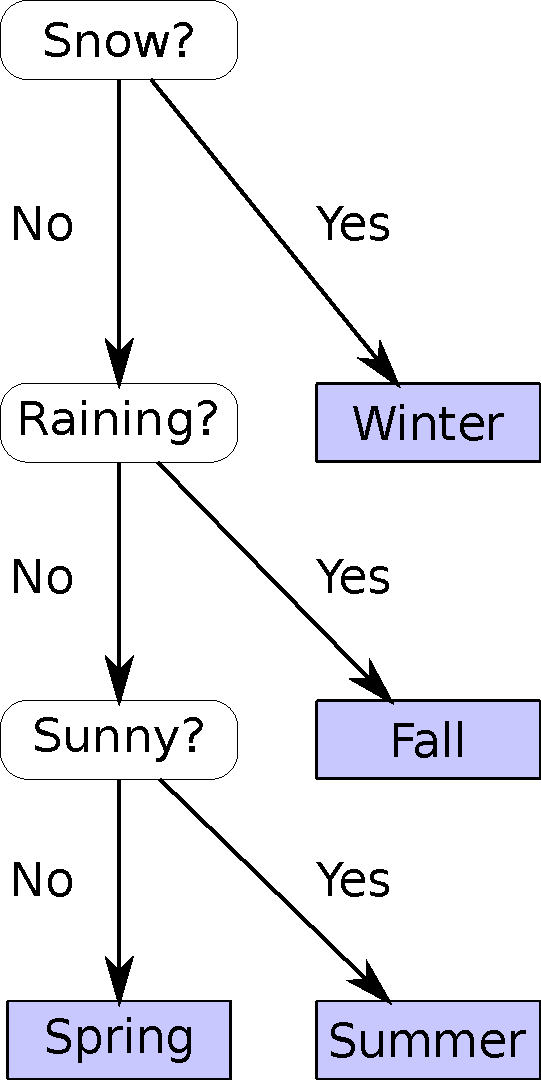
\includegraphics[width=0.8\columnwidth]{DecisionTree_partial.pdf}}
\vspace*{0.01cm}
\par 
{\scriptsize Decision Tree without the \emph{Temperature} attribute.\par}
\end{columns}
\end{frame}

\begin{frame}{Random Forest}
\begin{itemize}
\item The RF extracts values at randomly selected coordinates.
\item For example, if we have a data matrix $\X \in \R^{10\times 4}$ (\emph{i.e.,} 10 samples with 4 features each), we might train trees with the
following subsets of the data:
\begin{itemize}
\item \textbf{Tree 1:} Train using rows \{6,4,7,2,6,3\} and columns \{1,2,4\}
\item \textbf{Tree 2:} Train using rows \{1,10,2,1,7,9\} and columns \{1,3\}
\item \textbf{Tree 3:} Train using rows \{7,2,7,3,9,3\} and columns \{2\}
\item ...
\end{itemize}
\item Note that rows (samples) are sampled \emph{with replacement}, \emph{i.e.,} rows may appear more than once. 
\item Columns are sampled \emph{without replacement} (it does not make sense to repeat the same data).
\end{itemize}
\end{frame}

\begin{frame}{Random Forest}
\begin{columns}
\column{0.7\textwidth}
\begin{itemize}
\item After training many trees each with different samples and features, 
the RF predicts the class by taking the majority vote: what is the most 
frequent label.
\item The number of trees varies from a few dozen to few thousand---default in Python is 10.
\item The attached picture is produced by a 10-tree random forest.
\end{itemize}
\column{0.3\textwidth}
\centerline{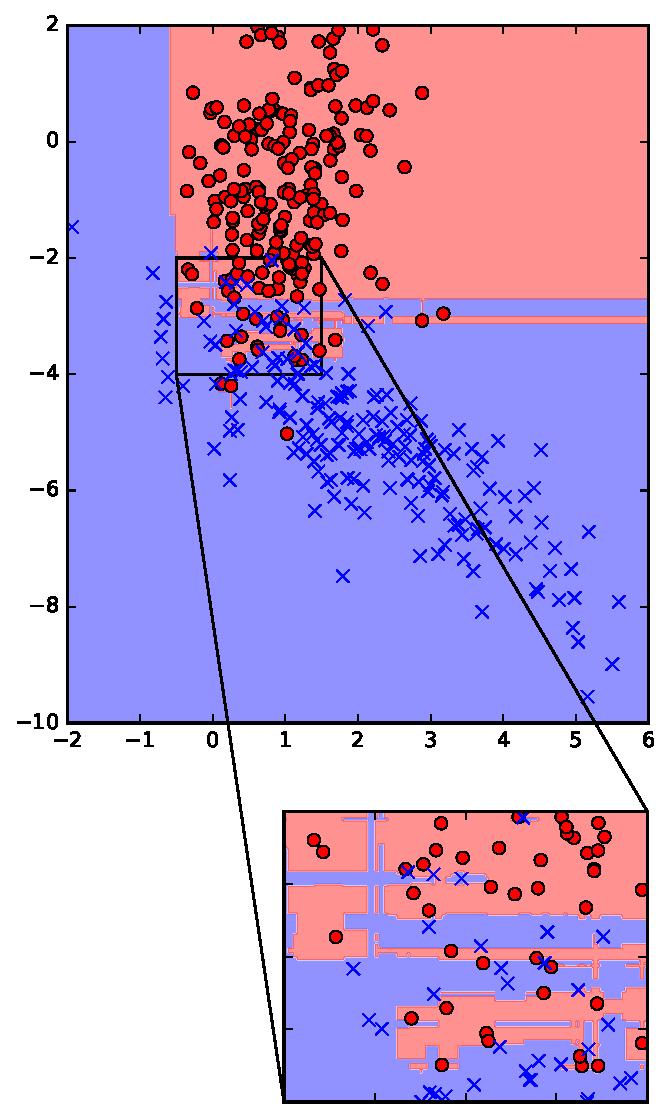
\includegraphics[width=1\columnwidth]{RandomForest1.pdf}}
\end{columns}
\end{frame}


\begin{frame}{Random Forest}
\begin{columns}
\column{0.75\textwidth}
\begin{itemize}
\item The collection of trees gives a natural way of estimating class
probabilities: Just use the proportion of trees voting for each class.
\item RF's also includes a method for assessing feature importances:
randomly shuffle each feature at a time
	and test how much the accuracy drops.
\end{itemize}
\vspace*{-0.2cm}
\begin{columns}[onlytextwidth]
\column{0.5\textwidth}
\begin{itemize}
\item Loosing an important feature drops the accuracy a lot.
\item Shuffling a non-important feature will not change the result much.
\end{itemize}
\column{0.5\textwidth}
\centerline{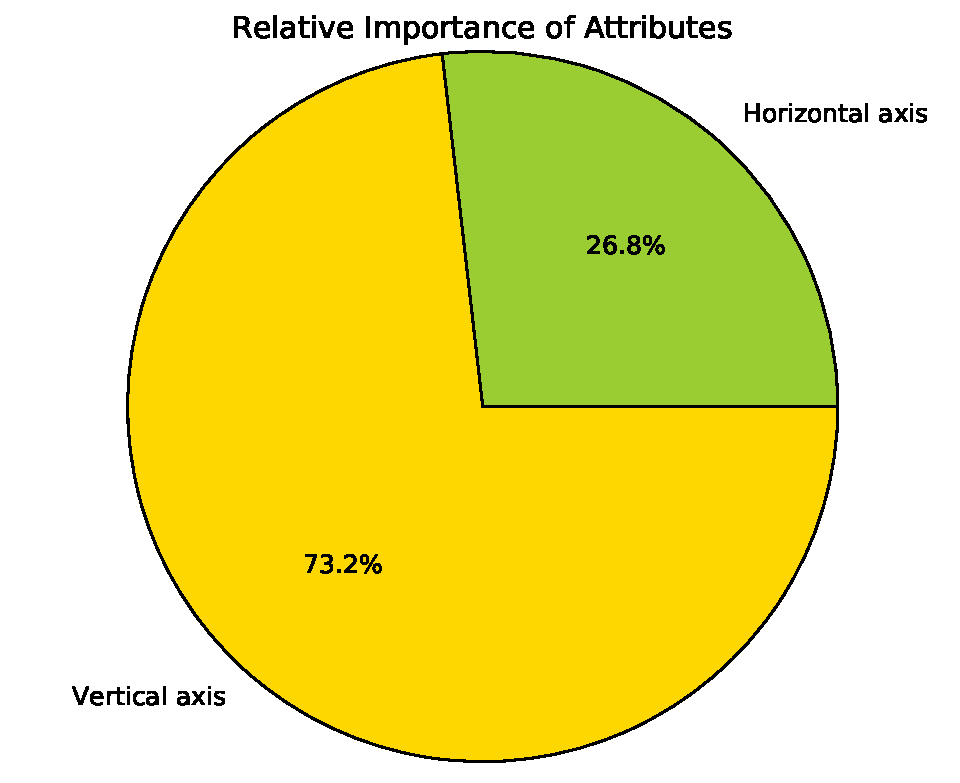
\includegraphics[width=\textwidth]{RF100_importances.pdf}}
\end{columns}
\column{0.3\textwidth}
\centerline{\includegraphics[width=1\columnwidth]{RF100_prob.pdf}}
\end{columns}
\end{frame}



\begin{frame}[fragile,allowframebreaks=0.8]
 {Random Forest in Scikit-Learn}
\begin{columns}[onlytextwidth]
\column{0.45\textwidth}
\begin{lstlisting}
# Training code:
from sklearn.ensemble import RandomForestClassifier

clf = RandomForestClassifier()
clf.fit(X, y)
\end{lstlisting}
\begin{lstlisting}
# Testing code:
>>>  clf.predict([0, -4])
array([ 0.])

>>>  clf.predict([0, -2])
array([ 1.])

>>> clf.predict_proba([[0, -4], [0, -2]])
array([[ 0.9,  0.1],
       [ 0.4,  0.6]])

>>> len(clf.estimators_)
10

>>> type(clf.estimators_[0])
sklearn.tree.tree.DecisionTreeClassifier
\end{lstlisting}
\column{0.6\textwidth}
\begin{itemize}
\item The \verb+RandomForestClassifier+ class is used via the normal interface (\verb+.fit()+ and \verb+.predict()+).
\item Individual trees can be accessed, as well: \verb+clf.estimators_+ is a list of \verb+DecisionTreeClassifier+
objects.
\item One of the 10 trained trees is visualized on the next slide (plot created using
\verb+sklearn.tree.export_graphviz+).
\end{itemize}
\end{columns}
\end{frame}

\begin{frame}[fragile]{Decision Tree}
\begin{center}
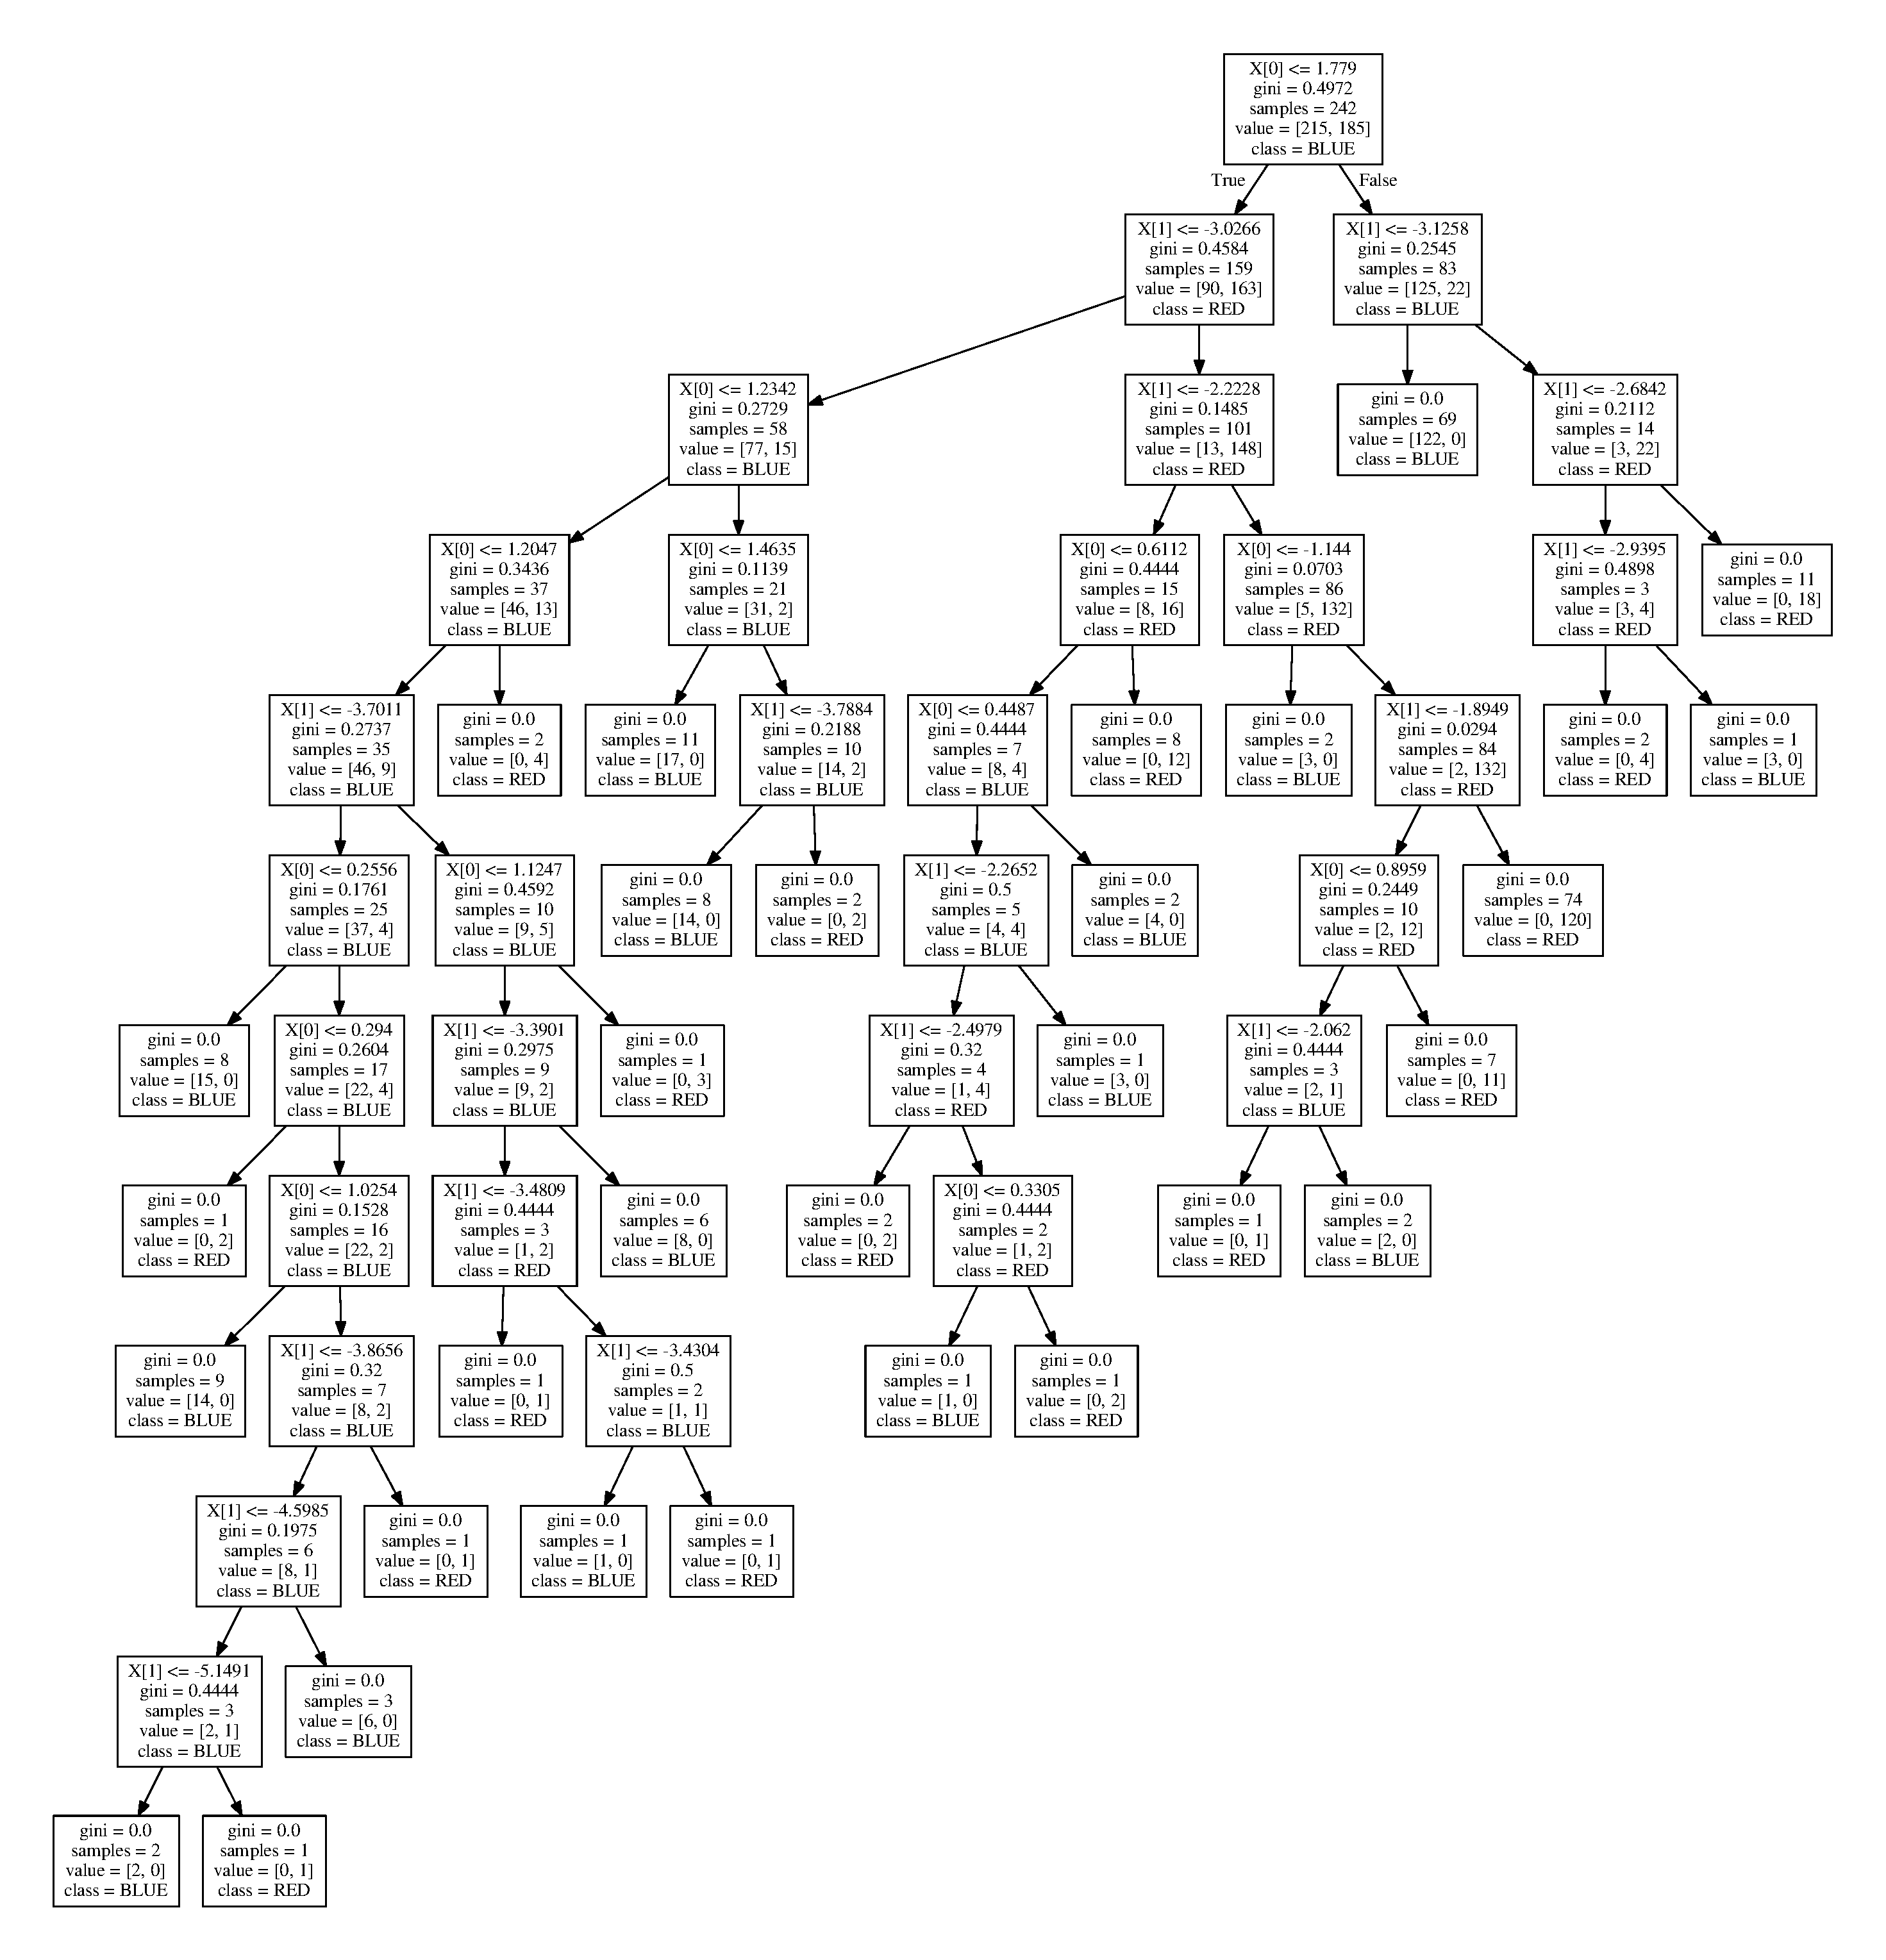
\includegraphics[width = 0.45\textwidth]{tree_graph_2.pdf}	\qquad
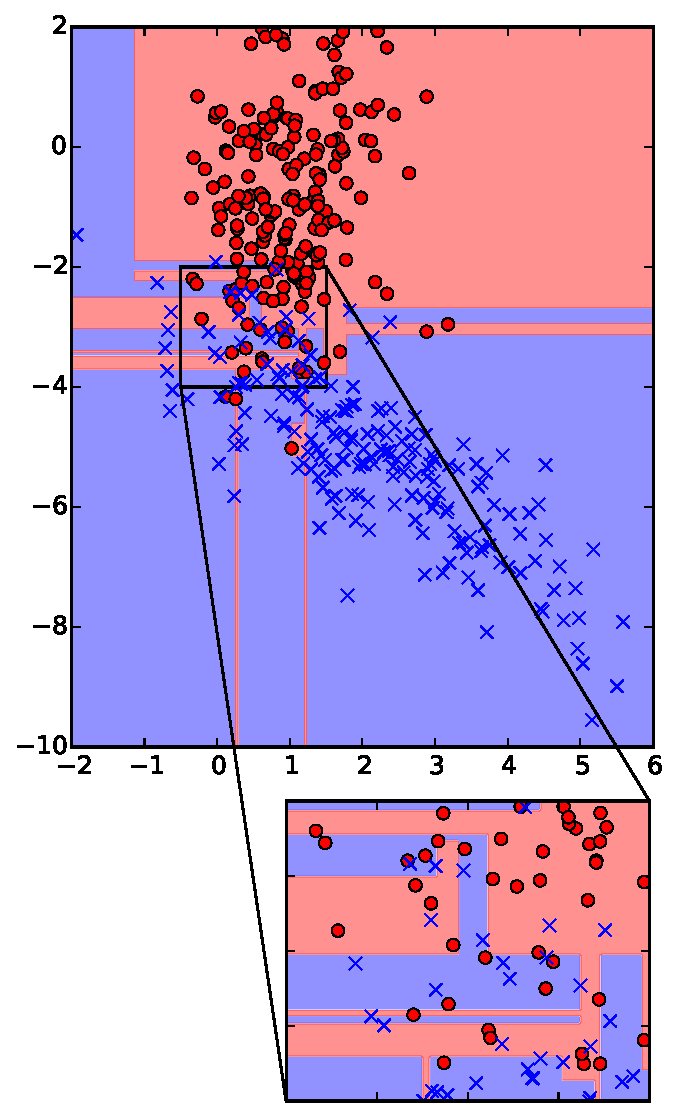
\includegraphics[width = 0.3\textwidth]{tree_2.pdf}	
\end{center}
\end{frame}


\begin{frame}[fragile, allowframebreaks=0.8]{Other Ensemble Classifiers}
\begin{itemize}
\item Since the introduction of Random Forest by Breiman in 1993, several extensions have been proposed.
\item As a group, these are called \emph{ensemble methods}, because they all consist of an ensemble of
weak classifiers,
\item Most important ones are briefly summarized in the following slides.
\end{itemize}
\end{frame}
	
\begin{frame}{AdaBoost Paradigm}
\begin{itemize}
	\item The \textbf{AdaBoost} paradigm
	was proposed 
	by Freund and Schapire in 1995. 
	\item Also in this case, the classifier consists of a collection of
	weak classifiers (most often decision trees). 
	\item The difference to other ensemble methods is that 
	trees are grown sequentially:
	\begin{enumerate}
		\item Assign each sample a weight $w_1\ldots,w_N$.
		\item Grow a tree minimizing the classification error 	
		weighted by $w_n$. That is, we emphasize the samples
		with large $w_n$.
		\item Append the new tree to our ensemble ${\cal E}$.
		\item Increase the weights for those samples that were incorrectly classified by ${\cal E}$.
		\item If not enough trees, then return to step 2.
	\end{enumerate}
	 \item Implemented as \texttt{sklearn.ensemble.AdaBoostClassifier}.
	\end{itemize}
	\end{frame}

		
\begin{frame}{Gradient Boosted Regression Trees}
\begin{itemize}
	\item \textbf{Gradient Boosted Regression Trees}
	were proposed by Friedman in 1999.
	\item Another boosting algorithm similar to AdaBoost.
	\item In this case, the training sequence is the following.
	\begin{enumerate}
		\item Initialize the ensemble ${\cal E}$ by a single decision tree fit to the data.
		\item Train another tree for correcting the errors made by ${\cal E}$, \emph{i.e.,} attempt to predict
		$\y - F_{\cal E}(\X)$.
		\item Append the new tree to our ensemble ${\cal E}$.
		\item If not enough trees, then return to step 2.
	\end{enumerate}
	\item Implemented as \texttt{sklearn.ensemble.GradientBoostingClassifier}.
	
\end{itemize}
	\end{frame}
		
\begin{frame}{Extremely Randomized Trees}
\begin{itemize}
	
	\item \textbf{Extremely Randomized Trees} were proposed by
	Geurts \emph{et al.} in 2006. 
	\item The idea is to make the trees even weaker, but to compensate that with the
	large number of estimators in the ensemble. 
	\item More specifically, not only the features and samples shown to the
	tree are randomized, but also the growing of individual trees is random.
	\item In particular the \emph{split point}
	\emph{i.e.,} the thresholds of comparisons like $X[1] <= -2.7025$ is randomized (see 
	the graph of a decision tree at an earlier slide.

\item Implemented as \texttt{sklearn.ensemble.ExtraTreesClassifier}.

\end{itemize}
\end{frame}


\begin{frame}[fragile]{Comparison of Methods}
\begin{columns}
\column{0.65\textwidth}
\begin{itemize}
	\item The four ensemble methods were compared with the \textbf{arcene dataset}:
	\url{https://archive.ics.uci.edu/ml/datasets/Arcene}.
	\item For randomized algorithms, we iterate the experiment 100 times.
\end{itemize}
\begin{lstlisting}
# Load Arcene data; 100+100 samples with dimension 10000:
# Mass spectrometer measurements from ovarian cancer patients and healthy controls.
X_train, y_train, X_test, y_test = load_arcene()

classifiers = [(RandomForestClassifier(), "Random Forest"),
               (ExtraTreesClassifier(), "Extra-Trees"),
               (AdaBoostClassifier(), "AdaBoost"),
               (GradientBoostingClassifier(), "GB-Trees")]
           
for clf, name in classifiers:
    clf.n_estimators = 100
    
    accuracies = []    
    for iteration in range(100):        
        clf.fit(X_train, y_train)
        y_hat = clf.predict(X_test)
        accuracy = accuracy_score(y_test, y_hat)
        accuracies.append(accuracy)
\end{lstlisting}
\column{0.25\textwidth}
\centerline{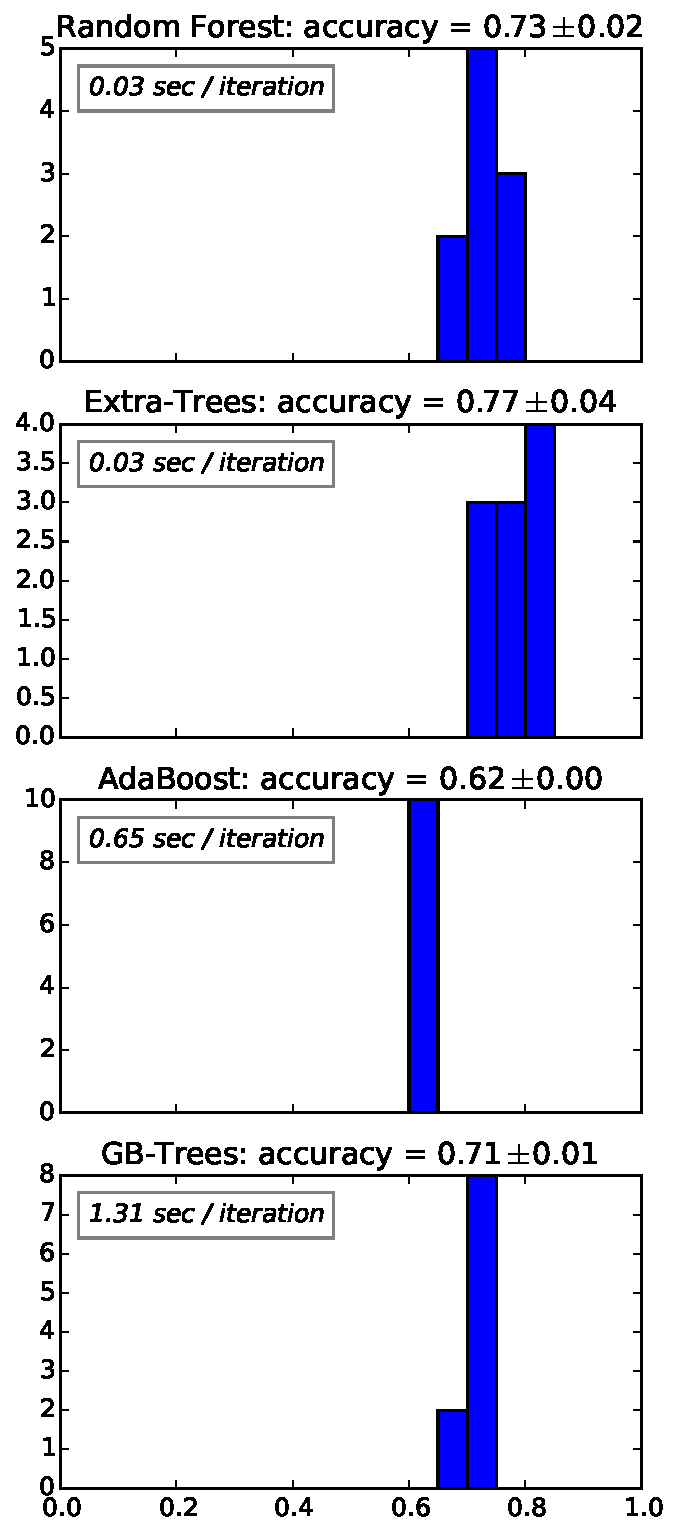
\includegraphics[width = \textwidth]{EnsembleComparison.pdf}}
\end{columns}
\end{frame}


\begin{frame}[fragile]{Comparison of Methods}
\begin{itemize}
	\item Let's add a bunch of other classifiers into our for loop.
	\begin{itemize}
		\item \emph{1-Nearest Neighbor}: \textbf{0.88}
		\item \emph{Logistic Regression}: 0.84
		\item \emph{Linear SVM}: 0.83
		\item \emph{5-Nearest Neighbor}: 0.82
		\item \emph{LDA}: 0.79
		\item \emph{Extra-Trees}: 0.77 $\pm$ 0.04
		\item \emph{9-Nearest Neighbor}: 0.73
		\item \emph{Random Forest}: 0.73 $\pm$ 0.02
		\item \emph{GB-Trees}: 0.71 $\pm$ 0.01
		\item \emph{AdaBoost}: 0.62		
		\item \emph{SVM with RBF kernel}: 0.56
	\end{itemize}
	\item It seems that linear models and NN excel with this data.
\end{itemize}
\end{frame}

\end{document}
\end{document}

